\documentclass[a4paper]{scrartcl}
\usepackage[english]{babel}
\usepackage[top=2cm,bottom=3cm,left=2.5cm,right=2.5cm]{geometry}
\usepackage[colorlinks=true, allcolors=black]{hyperref}
\usepackage{wrapfig} %문단 내 이미지 삽입
\usepackage{graphicx} %색상
\usepackage{overpic}
\usepackage[normalem]{ulem}%취소선
\usepackage{array} %표
\usepackage{mdframed, tcolorbox} %글상자
\usepackage[yyyymmdd]{datetime}
	\renewcommand{\dateseparator}{-}

\usepackage{amsmath, amsfonts, amssymb, bm} %수식
	\DeclareMathOperator{\arccsc}{arccsc}
	\DeclareMathOperator{\arcsec}{arcsec}
	\DeclareMathOperator{\arccot}{arccot}
	\DeclareMathOperator{\csch}{csch}
	\DeclareMathOperator{\sech}{sech}
	\DeclareMathOperator{\arcsinh}{arcsinh}
	\DeclareMathOperator{\arccosh}{arccosh}
	\DeclareMathOperator{\arctanh}{arctanh}
	\DeclareMathOperator{\arccsch}{arccsch}
	\DeclareMathOperator{\arcsech}{arcsech}
	\DeclareMathOperator{\arccoth}{arccoth}
	
	\DeclareMathOperator{\meter}{m}
	\DeclareMathOperator{\cm}{cm}
	\DeclareMathOperator{\mm}{mm}
	\DeclareMathOperator{\mum}{\mu m}
	\DeclareMathOperator{\newton}{N}
	\DeclareMathOperator{\kn}{kN}
	\DeclareMathOperator{\kgf}{kgf}
	\DeclareMathOperator{\pa}{Pa}
	\DeclareMathOperator{\kpa}{kPa}
	\DeclareMathOperator{\mpa}{MPa}
	\DeclareMathOperator{\gpa}{GPa}
	\DeclareMathOperator{\knpm}{kN/m}
	\DeclareMathOperator{\kph}{km/h}
	\DeclareMathOperator{\mps}{m/s}
	\DeclareMathOperator{\tkph}{kph}
	\DeclareMathOperator{\tmps}{mps}
	\DeclareMathOperator{\mpss}{m/s^2}
	\DeclareMathOperator{\dgr}{\!^\circ}
	\DeclareMathOperator{\cel}{\!^\circ C}
	\DeclareMathOperator{\kg}{kg}
	\DeclareMathOperator{\kgpcm}{kg/m^3}
	\DeclareMathOperator{\nm}{N\cdot m}
	\DeclareMathOperator{\kw}{kW}
	\DeclareMathOperator{\kwh}{kWh}
	\DeclareMathOperator{\mmhg}{mmHg}
	\DeclareMathOperator{\snd}{s}
\usepackage{polynom} %나눗셈 필산
\usepackage{cancel} %수식 약분선
\usepackage{titlesec} %섹션 이름 변경
	\titlespacing*{\section}{3mm}{0mm}{1mm}
	\titleformat{\section}{\bfseries\large}{}{0ex}{}
\usepackage{kotex} %한글

\newcommand{\prob}[2]{\section{#1}\begin{mdframed}#2\end{mdframed}}

\newlength{\picwidth}
\newcommand{\probpic}[4]{
	\setlength{\picwidth}{145mm}\addtolength{\picwidth}{-#3}\section{#1}\begin{mdframed}\begin{tabular}{m{#3}m{\picwidth}}
			\includegraphics[width = #3]{#2} & #4\end{tabular}\end{mdframed}
}

\newcommand{\asw}[2]{
	\begin{flushright}
		#1\quad$\blacktriangleleft$\quad#2
	\end{flushright}
}

\newcommand{\aswtag}[1]{
	\quad\blacktriangleleft\quad#1
}

\title{\vspace{100pt}\Huge{HW5}}
\author{
	2025-1 고체역학(박성훈 교수님)\\[10pt]
	Concept Aplication 4.7, Problem 4.1, 4.16, 4.24, 4.33, 4.67, 4.91, 4.100\\[100pt]
	오류 제보 : eunsoohong03@soongsil.ac.kr\\
	}
\date{\today}

\begin{document}
	
\renewcommand*{\titlepagestyle}{empty}
\maketitle
\setlength{\parindent}{0pt}

\vspace{60pt}

\begin{center}
	\includegraphics[width=0.45\textwidth]{SSU symbol KR-EN.jpg}
\end{center}

\newpage
\setcounter{page}{1}

\section{Concept Aplication 4.7}
	\begin{mdframed}
		\begin{tabular}{m{35mm}m{110mm}}
			\includegraphics[width = 35mm]{img/ca4-7.png}
			&
			An open-link chain is obtained by bending low-carbon steel rods of 12-mm diameter into the shape shown (Fig. 4.43a). Knowing that the chain carries a load of 700 N, determine ($a$) the largest tensile and compressive stresses in the straight portion of a link, ($b$) the distance between the centroidal and the neutral axis of a cross section.
		\end{tabular}
	\end{mdframed}
	\begin{align*}
		&A = \pi(0.006)^2\meter^2 = 1.130973\times10^{-4}\meter^2,\quad I = \frac{\pi}{4}(0.006)^4\meter^4 = 1.017876\times10^{-9}\meter^4\\
		&M = Fd = (700)(0.016)\nm = 11.2\nm\\
		&\sigma = \sigma_\text{axial loading} + \sigma_\text{bending} = \frac{P}{A} - \frac{Mx}{I}\\
		&\frac{P}{A} = \frac{700}{1.130973\times10^{-4}}\pa = 6.18936\mpa,\quad \frac{Mc}{I} = \frac{(11.2)(0.006)}{1.017876\times10^{-9}}\pa = 66.0198\mpa\\[5pt]
		&\left.\begin{array}{l}
			\sigma_{\text{max}} = \cfrac{P}{A} + \cfrac{Mc}{I} = 72.2\mpa\\[10pt]
			\sigma_{\text{min}} = \cfrac{P}{A} - \cfrac{Mc}{I} = -59.8\mpa
		\end{array}\right\}\aswtag{(a)}\\[5pt]
		&0 = \cfrac{P}{A} - \frac{Mx_n}{I}\quad\Rightarrow\quad x_n = \frac{PI}{MA} = \frac{(700)(1.017876\times10^{-9})}{(11.2)(1.130973\times10^{-4})}\meter = 0.563\mm\aswtag{(b)}
	\end{align*}

\vspace{20pt}

\section{Problem 4.1}
	\begin{mdframed}
		Knowing that the couple shown acts inavertical plane, determine the stress at ($a$) point $A$. ($b$) point $B$.\\
		\phantom{.}\hspace{45mm}\includegraphics[width = 65mm]{img/p4-1.png}
	\end{mdframed}
	\begin{align*}
		&I = \frac{\pi}{4}\left(0.02^4 - 0.015^4\right)\meter^4 = 8.59029\times10^{-8}\meter^4\\
		&\sigma_A = -\frac{Mc}{I} = -\frac{(500)(0.02)}{8.59029\times10^{-8}}\pa = -116.4\mpa\aswtag{(a)}\\
		&\sigma_B = -\frac{My_{\text{in}}}{I} = -\frac{(500)(0.015)}{8.59029\times10^{-8}}\pa = -87.3\mpa\aswtag{(b)}
	\end{align*}

\newpage

\section{Problem 4.16}
	\begin{mdframed}
		The beam shown is made of a nylon for which the allowable stress is 24 MPa in tension and 30 MPa in compression. Determine the largest couple $\mathbf{M}$ that can be applied to the beam.
		\begin{center}
			\includegraphics[width = 95mm]{img/p4-16.png}
		\end{center}
	\end{mdframed}
	\begin{align*}
		&A_1 = (40\mm)(15\mm) = 600\mm^2,\quad A_2 = (20\mm)(15\mm) = 300\mm^2\\
		&\bar{y}_1 = \frac{15\mm}{2} = 7.5\mm,\quad \bar{y}_2 = 15\mm + \frac{15\mm}{2} = 22.5\mm\\
		&\bar{y} = \frac{\bar{y}_1A_1 + \bar{y}_2A_2}{A_1 + A_2} = \frac{(7.5)(600) + (22.5)(300)}{600+300}\mm = 12.5\mm\\
		&I_1 = \frac{1}{12}(40)(15)^3\mm^4 = 11250\mm^4,\quad I_2 = \frac{1}{12}(20)(15)^3\mm^4 = 5625\mm^4\\
		&I = I_1 + A_1(\bar{y}_1 - \bar{y})^2 + I_2 + A_2(\bar{y}_2 - \bar{y})^2 = 61875\mm^4 = 6.1875\times10^{-8}\meter^4\\
		&\sigma_\text{max} = \frac{My_\text{max}}{I} \leq \sigma_{t,\text{all}},\quad M \leq \frac{\sigma_{t,\text{all}}I}{y_\text{max}} = \frac{(24\times10^6)(6.1875\times10^{-8})}{0.0125}\nm = 118.8\nm\\
		&|\sigma_\text{min}| = \frac{M|y_\text{min}|}{I} \leq \sigma_{c,\text{all}},\quad M \leq \frac{\sigma_{c,\text{all}}I}{|y_\text{min}|} = \frac{(30\times10^6)(6.1875\times10^{-8})}{0.0125}\nm = 106.1\nm\\
		&\Rightarrow\quad M_m = 106.1\nm\aswtag{}
	\end{align*}
	
\newpage

\section{Problem 4.24}
	\begin{mdframed}
	\begin{tabular}{m{50mm}m{95mm}}
		\includegraphics[width = 50mm]{img/p4-24.png}
		&
		A 60-N-m couple is applied to the steel bar shown. ($a$) Assuming that the couple is applied about the $z$ axis as shown, determine the maximum stress and the radius of curvature of the bar. ($b$) Solve part $a$, assuming that the couple is applied about the $y$ axis. Use $E=200\gpa$.
	\end{tabular}
	\end{mdframed}
	Solving ($a$),
	\begin{align*}
		&I = \frac{1}{12}(12\mm)(20\mm)^3 = 8000\mm^4\\
		&\sigma_m = \frac{Mc}{I} = \frac{(60\nm)(10\mm)}{8000\mm^4} = \frac{60\times10}{8000}\times10^3 \mpa = 75.0\mpa\quad\cdots\quad(a)-1\\
		&\varepsilon_m = -\frac{c}{\rho}\\
		&\rho = -\frac{c}{\varepsilon_m} = -\frac{cE}{\sigma_m} = \frac{(10\mm)(200\gpa)}{75\mpa} = \frac{10\times200}{75}\meter = 26.7\meter\quad\cdots\quad(a)-2
	\end{align*}
	Solving ($b$),
	\begin{align*}
		&I = \frac{1}{12}(20\mm)(12\mm)^3 = 2880\mm^4\\
		&\sigma_m = \frac{Mc}{I} = \frac{(60\nm)(6\mm)}{2880\mm^4} = \frac{60\times6}{2880}\times10^3 \mpa = 125.0\mpa\quad\cdots\quad(b)-1\\
		&\rho = -\frac{c}{\varepsilon_m} = -\frac{cE}{\sigma_m} = \frac{(6\mm)(200\gpa)}{125\mpa} = \frac{6\times200}{125}\meter = 9.60\meter\quad\cdots\quad(b)-2
	\end{align*}

\newpage

\section{Problem 4.33}
    \begin{mdframed}
    \begin{tabular}{m{45mm}m{100mm}}
    	\begin{tabular}{l}
        	\includegraphics[width = 45mm]{img/p4-33.png}
   		\end{tabular}
        &
        \begin{tabular}{m{95mm}}
            A bar having the cross section shown has been formed by securely
            bonding brass and aluminum stock. Using the data given in the table,
            determine the largest permissible bending moment when the composite bar is
            bent about a horizontal axis.\\
            \centering
			\includegraphics[width = 65mm]{img/p4-33-1.png}
        \end{tabular}
    \end{tabular}
    \end{mdframed}
    \begin{align*}
    	&n = \frac{E_\text{br}}{E_\text{Al}} = \frac{105\gpa}{70\gpa} = 1.5
    \end{align*}
    \includegraphics{img/p4-33-2.png}
    \begin{align*}
    	&I_R = \frac{1}{12}(45)(42)^3 - \frac{1}{12}(15)(30)^3\;[\mm^4] = 244080\mm^4\\
    	&\sigma_{m,\text{Al}} = \frac{My_{\text{Al}}}{I_R} \leq \sigma_{\text{all,Al}},\quad M\leq \frac{\sigma_{\text{all,Al}}I_R}{c_{\text{Al}}} = \frac{(100\mpa)(244080\mm^4)}{15\mm} = 1.627\kn\cdot\meter\\
    	&\sigma_{m,\text{br}} = n\frac{Mc}{I_R} \leq \sigma_{\text{all,br}},\quad M\leq \frac{\sigma_{\text{all,br}}I_R}{nc} = \frac{(160\mpa)(244080\mm^4)}{1.5(21\mm)} = 1.240\kn\cdot\meter\\
    	&\Rightarrow\quad M_{\text{max}} = 1.240\kn\cdot\meter
    \end{align*}

\vspace{20pt}

\section{Problem 4.67}
	\begin{mdframed}
		\begin{tabular}{m{45mm}m{100mm}}
			\includegraphics[width = 45mm]{img/p4-67.png}
			&
			A bar of rectangular cross section, made of a steel assumed to be elastoplastic with $\sigma_y = 320\mpa$, is subjected to a couple $M$ parallel to the $z$ axis. Determine the moment $M$ of the couple for which ($a$) yield first occurs, ($b$) the plastic zones at the top and bottom of the bar are 5 mm thick.
		\end{tabular}
	\end{mdframed}
	\begin{align*}
		&M_Y = \frac{2}{3}\sigma_Ybc^2 = \frac{2}{3}(320\mpa)(12\mm)(7.5\mm)^2 = 144.0\nm\quad\cdots\quad(a)\\
		&M = \frac{3}{2}M_Y\left(1-\frac{y_Y^2}{3c^2}\right) = \frac{3}{2}(144\nm)\left(1- \frac{2.5^2}{3(7.5)^2}\right) = 208\nm\quad\cdots\quad(b)
	\end{align*}
	
\newpage

\section{Problem 4.91}
	\begin{mdframed}
		\begin{tabular}{m{35mm}m{110mm}}
			\includegraphics[width = 35mm]{img/p4-91.png}\newline \tiny{image generated by ChatGPT}
			&
			A bending couple is applied to the beam of Prob. 4.73($E = 200\gpa,\;\sigma_Y = 240\mpa$), causing plastic zones $30\mm$ thick to develop at the top and bottom of the beam. After the couple has been removed, determine ($a$) the residual stress at $y = 45\mm$, ($b$) the points where the residual stress is zero, ($c$) the radius of curvature corresponding to the permanent deformation of the beam.
		\end{tabular}
	\end{mdframed}
	\begin{align*}
		&I = \frac{1}{12}(60)(90)^3\mm^4 = 3.645\times10^{-6}\meter^4\\
		&M_Y = \frac{2}{3}\sigma_Ybc^2 = \frac{2}{3}(240\mpa)(60\mm)(45\mm)^2 = 19.44\kn\cdot\meter\\
		&M = \frac{3}{2}M_Y\left(1 - \frac{y_Y^2}{3c^2}\right) = \frac{3}{2}(19.44\kn\cdot\meter)\left(1 - \frac{15^2}{3(45)^2}\right) = 28.08\kn\cdot\meter\\
		&\sigma_m'= \frac{Mc}{I} = \frac{(28.08\kn\cdot\meter)(0.045\meter)}{3.645\times10^{-6}\meter^4} = \frac{1040}{3}\mpa\\
		&\sigma_{\text{res}}|_{y = 45\mm} = -\sigma_Y +\sigma_m' = -240\mpa + \frac{1040}{3}\mpa = 106.7\mpa\quad\cdots\quad(a)\\
		&0 = -\sigma_Y + \frac{y\sigma_m'}{c},\quad y = c\frac{\sigma_Y}{\sigma_m'} = (45\mm)\frac{240\mpa}{\frac{1040}{3}\mpa} = 31.2\mm,\quad y = \pm31.2\mm\quad\cdots\quad(b)\\
		&\sigma_{\text{res},Y} = -\sigma_Y + \frac{y_Y\sigma_m'}{c} = -240\mpa + \frac{(15\mm)(\frac{1040}{3}\mpa)}{45\mm} = -\frac{1120}{9}\mpa\\
		&\rho_p = -\frac{y_Y}{\varepsilon_Y} = -\frac{y_YE}{\sigma_{\text{res},Y}} = -\frac{(15\mm)(200\gpa)}{-\frac{1120}{9}\mpa} = 24.1\meter\quad\cdots\quad(c)
	\end{align*}

\vspace{20pt}

\section{Problem 4.100}
	\begin{mdframed}
		\begin{tabular}{m{50mm}m{95mm}}
			\includegraphics[width = 50mm]{img/p4-100.png}
			&
			Knowing that the magnitude of the vertical force $P$ is $8\kn$, determine the stress at ($a$) point $A$, ($b$) point $B$.
		\end{tabular}
	\end{mdframed}
	\begin{align*}
		&I = \frac{1}{12}(30)(24)^3\mm^4 = 3.456\times10^{-8}\meter^4\\
		&M = (8\kn)(45\mm-12\mm) = 264\nm\\
		&\sigma = \sigma_{\text{loading}} + \sigma_{\text{bending}} = \frac{P}{A} + \frac{My}{I}\\
		&\sigma_A = \frac{-8000\newton}{(0.03\meter)(0.024\meter)} + \frac{(264\nm)(-0.012\meter)}{3.456\times10^{-8}\meter^4} = -102.8\mpa\\
		&\sigma_B = \frac{-8000\newton}{(0.03\meter)(0.024\meter)} + \frac{(264\nm)(0.012\meter)}{3.456\times10^{-8}\meter^4} = 80.6\mpa
	\end{align*}


\end{document}